\documentclass[twocolumn]{article}

\usepackage{geometry}
\geometry{textwidth = 18cm,textheight = 24cm}

\usepackage{cite}
\usepackage{caption}
\usepackage{graphicx}
\usepackage{amsmath}
\usepackage{amssymb}
%\usepackage{braket}
\usepackage{textcomp}
%\usepackage{lmodern}
\usepackage{authblk}
\usepackage{datetime}
\usepackage{gensymb}
\usepackage{wrapfig}
%\usepackage[usenames,dvipsnames,svgnames,table]{xcolor}
\usepackage{booktabs}
%\usepackage{appendix}

%\usepackage[switch,columnwise]{lineno}
%\linenumbers

\newcommand{\onlinecite}[1]{\hspace{-1 ex} \nocite{#1}\citenum{#1}} 

\let\OLDthebibliography\thebibliography
\renewcommand\thebibliography[1]{
  \OLDthebibliography{#1}
  \setlength{\parskip}{0pt}
  \setlength{\itemsep}{0pt plus 0.3ex}
}
  
\title{Modeling Loop Neurons as Systems of Coupled Leaky Integrators}
\author[1]{\Large{NIST Physics and Hardware for Intelligence Project}
\\
\textit{\large{National Institute of Standards and Technology}}
\\
\vspace{-0.2em}
\textit{\large{325 Broadway, Boulder, CO, USA, 80305}}
\\
\vspace{-0.2em}
\textit{\large{jeffrey.shainline@nist.gov}}
}
\date{\today}%\today

\begin{document}

\twocolumn[
  \begin{@twocolumnfalse}
    \maketitle
    \begin{abstract}

Superconducting optoelectronic loop neurons are a class of circuits potentially conducive to realizing networks for large-scale artificial cognition. These circuits employ superconducting components including single-photon detectors, Josephson junctions, and transformers. To date, all simulations of loop neurons have used first-principles circuit analysis to model the behavior of synapses, dendrites, and neurons. These circuit models are computationally inefficient and leave opaque the relationship between loop neurons and other neuron models employed in computational neuroscience and cognitive computing. Here we introduce a modeling framework that captures the behavior of the relevant synaptic, dendritic, and neuronal circuits at a phenomenological level without resorting to full solutions to the circuit equations. In this framework, each synapse and dendrite is discovered to obey a single leaky-integrator ordinary differential equation, while a neuron with adaptive refraction is modeled as two dendrites in a feedback configuration. We quantify the accuracy of the phenomenological model relative to circuit simulations, and find that the approach not only reduces the total number of differential equations in the coupled system, but also allows an increase in the numerical time step by a factor of 100. We demonstrate the use of the model with several basic examples. The net increase in computational efficiency enables future simulation of large, interconnected networks, while the formulation in terms of well-known leaky integrators provides a connection to a large body on work in applied mathematics and computational neuroscience, which aids in development of intuition for the operation of future superconducting optoelectronic networks.

    \vspace{3em}
    \end{abstract}
  \end{@twocolumnfalse}
]

\setcounter{tocdepth}{1}
\setcounter{secnumdepth}{4}
%\tableofcontents

\section{\label{sec:introduction}Introduction}

% this introduction is too long-winded
Comprehensive knowledge of large-scale neural systems is a grand scientific challenge with relevance to neuroscience, artificial intelligence, and the physics of critical systems \cite{elst2012,ized2008,br2017,fama2019,eide2019}. The lack of an efficient, artificial, brain-scale experimental test bed is a barrier to progress. Experiments with living systems bring challenges, including the difficulty of obtaining data from large numbers of individual neurons, let alone synapses. Data acquired at the scale of the entire network has low resolution, while it is difficult to obtain data with high spatial and temporal resolution at the device and network levels simultaneously. The invasive nature of experiments on functioning systems is also problematic. The ability to adjust device, circuit, and network parameters of biological neural systems is limited, limiting the potential of controlled experiments. An artificial platform capable of realizing networks at the scale and complexity of the brains of intelligent organisms would be a tool of supreme scientific utility.

Neuromorphic hardware based on silicon microelectronics has a great deal to offer in this regard \cite{me1989,lide2015,chba2003,inch2006,voma2007,inli2011,cryu2012,cage2013,pfgr2013,bega2014,fu2016,moqi2018}. Yet challenges remain. Silicon neural circuits cannot directly communicate via axons in the manner of biological neurons, so communication is carried out over shared circuits comprising an interconnection network. Bottlenecks result that make information integration across space and time less efficient than biological neural systems. Additionally, adaptation and learning are hindered by difficulties with mechanisms for storing and writing a memory state in devices monolithically integrated with the MOSFETs performing neural computations. While the decades of progress developing silicon neural circuits have achieved impressive gains, as a test bed for cognition, alternative hardware may bring new benefits.

Many proposals have arisen to explore alternative hardware for cognition, including using optical \cite{psfa1985,faps1985,abps1987,waps1993,safi1995,mosc1997,hoiz2000,moho2000,rokr2009,krfo2011,dusc2012,nash2013,prsh2017,shha2017,pena2018,tafe2019} and magnetic \cite{} phenomena as well as phase-change materials \cite{chsa2019,feyo2019}. It has been argued that using optical pulses to represent action potentials may alleviate the need for a shared communication infrastructure and the associated demands on address storage and memory access \cite{shbu2017,sh2019}. The use of superconducting circuits bring the thresholding nonlinearity of Josephson junctions \cite{vatu1998,ka1999} as well as memory retention and plasticity through the storage of flux in superconducting loops \cite{sh2019}. By using superconducting detectors \cite{nata2012} in conjunction with optical pulses, neurons can signal to synapses at the single-photon level. In conjunction with minimal static power dissipation, the energy efficiency of such systems may be conducive to very large artificial cognitive systems. Although the constituent devices dwarf their biological counterparts, communication at the speed of light enables a very large neuronal pool \cite{sh2019,sh2018_ICRC}. The apparent circuit complexity and adaptability are intriguing for scientific study.

% consider starting close to here
While the components of these superconducting optoelectronic networks (SOENs) have been demonstrated, full circuits have not. Prior to undertaking the full effort and expense of realizing these complex systems, it is prudent to gain confidence they are indeed ripe for further investigation. This confidence can be gained through simulations of device, circuit, and system behavior using conventional numerical methods. The computations performed by superconducting optoelectronic loop neurons are accomplished by circuits comprising superconducting single-photon detectors, Josephson junctions, and mutual inductors. These devices are most commonly modeled with SPICE circuit simulations carried out on a picosecond time scale to accurately capture the dynamics of the Josephson junctions. Simulation of networks of large numbers of these neurons become computationally intensive. From the perspective of the neural system, the picosecond dynamics of the JJs are not the primary interest, and one would prefer to treat each synapse, dendrite, and neuron as an input-output device with a model that accurately captures the circuit dynamics on the nanosecond to microsecond time scales while not explicitly treating the picosecond behavior of the underlying circuit elements.

Here we introduce a phenomenological model of loop neurons and their constitutive elements that accurately captures the transfer characteristics of the circuits without solving the underlying circuit equations. Each synapse and dendrite is treated with a single, first-order ordinary differential equation that describes the output of the element as a function of its inputs and instantaneous internal state. These equations take the standard form of a leaky integrator with a nonlinear driving term. Each neuron performs passive summation of its synaptic and dendritic inputs. When the sum of the inputs reaches threshold, the neuron produces a spike. Refraction is treated with the same formalism as a strong inhibitory synapse receiving the neuron's spikes and directly contacting the neuron's cell body. When full circuit simulations are conducted, each synapse or dendrite require solving a system of seven equations at each time step, and time steps of 1\,ps are typical. The model presented here reduces the number of equations for each synapse or dendrite to one and allows simulation with time steps of 1\,ns. 

We begin by motivating the form of the model based on circuit considerations. We then describe the means by which the form of the driving term in the leaky integrator is obtained. Error is quantified by comparison with full circuit simulations, and convergence is investigated as a function of time step size. Point neurons are considered to test the synaptic equations. Dendrites are treated next, and the similarity between synaptic and dendritic circuits permits a treatment with a similar form of leaky integrator equation. Dendritic accuracy is quantified, and an example of a neuron with a dendritic arbor is presented to illustrate the utility of the model. Throughout the work we compare and contrast loop neurons with their biological counterparts. 

\section{\label{sec:loop_neurons}Overview of Loop Neurons}
\begin{figure}[h!]
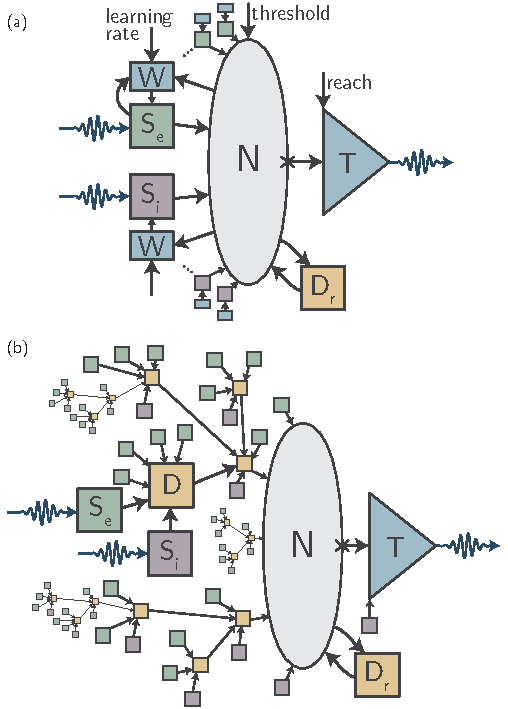
\includegraphics[width=8.6cm]{figures/_fig__schematics.pdf}
\captionof{figure}{\label{fig:schematic__circuits}Two schematics of loop neurons. (a) Schematic of a point loop neuron (no dendritic tree) \cite{sh2018,sh2019} showing excitatory ($\mathsf{S_e}$) and inhibitory ($\mathsf{S_i}$) synapses, as well as synaptic weight update circuits ($\mathsf{W}$). The wavy, colored arrows are photons, and the black arrows are electrical signals. The synapses receive signals as faint as a single photon and add supercurrent to an integration loop. Upon reaching threshold, a signal is sent to the transmitter circuit ($\mathsf{T}$), which produces a pulse of photons that are sent to downstream synaptic connections. Electrical signals generated by synapses and the neuron cell body are used for synaptic weight updates. A refractory dendrite ($\mathsf{D_r}$) receives spike outputs from the neuron and provides feedback to the neuron to accomplish adaptive refraction. (b) A loop neuron with an elaborate dendritic tree \cite{sh2020}. The complex structure consists of excitatory and inhibitory synapses that feed into dendrites ($\mathsf{D}$). Each dendrite performs computations on the inputs and communicates the result to other dendrites for further processing or on to the cell body of the neuron ($\mathsf{N}$). The neuron itself acts as the final thresholding stage, and when its threshold is reached, light is produced by the transmitter ($\mathsf{T}$), which is routed to downstream synaptic connections.}
\end{figure}

Research in superconducting optoelectronic networks of loop neurons aspires to realize artificial neural systems with scale and complexity comparable to the human brain. We have introduced the concepts of loop neurons in a number of papers \cite{sh2018,sh2019,sh2020}, and we have demonstrated many of the principles experimentally \cite{buch2017,chbu2017,chbu2018,mcve2019}. Schematic diagrams of two types of loop neuron are shown in Fig.\,\ref{fig:schematic}. Figure \ref{fig:schematic}(a) shows the point-neuron concept \cite{sh2018,sh2019_jap}, while Fig.\,\ref{fig:schematic}(b) shows the concept when a dendritic tree is included \cite{sh2019_jstqe}. In these neurons, integration, synaptic plasticity, and dendritic processing are implemented with inductively coupled loops of supercurrent. It is due to the prominent role of superconducting storage loops that we refer to devices of this type as loop neurons. 

Operation of loop neurons is as follows. Photons from upstream neurons are received by a superconducting single-photon detector (SPD) at each synapse. Using a Josephson junction (JJ) in parallel with an SPD, synaptic detection events are converted into an integrated supercurrent which is stored in a superconducting loop. The circuit diagram of a synapse is shown in Fig.\,\ref{fig:circuits}(a). The amount of current that gets added to the integration loop during a photon detection event is determined by the synaptic weight. The synaptic weight is dynamically adjusted by another circuit combining SPDs and JJs, and all involved circuits are analog. When the integrated current of a given neuron reaches a (dynamically variable) threshold, an amplification cascade begins, resulting in the production of light from a waveguide-integrated semiconductor light emitter. The photons thus produced fan out through a network of dielectric waveguides and arrive at the synaptic terminals of other neurons where the process repeats.

In loop neurons, a synapse consists of an SPD in parallel with a JJ (which together transduce photons to supercurrent), and a superconducting loop, which stores a current proportional to the number of detected photon arrival events. This loop is referred to as the synaptic integration (SI) loop. Within each neuron, the loops of many synapses are inductively coupled to a larger superconducting loop, referred to as the neuronal receiving (NR) loop, thereby inducing an integrated current proportional to a weighted sum of the currents in all the neuron's synapses. When the current in this NR loop reaches a threshold, the neuron produces a current pulse in the form of one or more flux quanta. This current is amplified and converted to voltage to produce photons from a semiconductor $p-i-n$ junction.

The currents in the synaptic and neuronal loops are analogous to the membrane potential of biological neurons \cite{daab2001,geki2002}, and the states of flux in these loops are the principal dynamical variables of the synapses and neurons in the system. Inhibitory synapses can be achieved through mutual inductors with the opposite sign of coupling. Dendritic processing can be implemented straightforwardly by adding intermediate mutually inductively coupled loops between the synaptic and neuronal loops. Synapses can be grouped on dendritic loops capable of local, nonlinear processing and inhibition. Neurons with multiple levels of dendritic hierarchy can be implemented as multiple stages of integrating loops. The temporal scales of the SI and DI loops can be set with $L/r$ time constants. I expect all synaptic and dendritic signals to leak, enabling fading memory of recent activity. Also, I hypothesize that the ability to achieve a diversity of time constants through synapses and dendrites with many $L/r$ time constants will be advantageous, and I would like to investigate this in numerical studies.

Synaptic memory is also implemented based on the stored flux in a loop, referred to as the synaptic storage (SS) loop. The state of flux in the SS loop determines the current bias to the synaptic receiver circuit discussed above. This current bias is the synaptic weight. In contrast to the SI and DI loops, the SS loop is intended to store long-term memory, and therefore I do not expect to add a resistance to this loop. If the SS loop is created with a superconducting wire of high inductance, the loop can hold many discrete states of flux, and therefore can implement many synaptic weights, if desired. Synapses with a pseudo-continuum of hundreds of stable synaptic levels between minimal and maximal saturation values are possible. Transitions between these levels can be induced based on the relative arrival times of photons from the pre-synaptic and post-synaptic neurons, thereby establishing a means for spike-timing-dependent plasticity with one photon required for each step of the memory-update process. Binary synapses are also possible, and just as we expect a diversity of $L/r$ time constants to be advantageous for tracking activity over time, we expect a diversity of synapses raging from binary to multistable to be advantageous for striking a balance between adaptability and long-term memory retention.

A primary goal of developing the phenomenological model presented here is to elucidate similarities and differences between loop neurons and well-studied leaky integrate-and-fire (LIF) neurons. 



\section{\label{sec:leaky_integrators}Context of the Model: Leaky Integrators}
\begin{equation}
\label{eq:leaky_integrator}
\frac{dQ(t)}{dt} = f(t)-\frac{Q(t)}{\tau},
\end{equation}
The general form of a leaky integrator differential equation is given in Eq.\,\ref{eq:leaky_integrator}. This equation can model many physical systems wherein a quantity of interest accumulates in time due to a driving function $f(t)$ while also leaking exponentially with a time constant $\tau$. 


\section{\label{sec:synapses}Loop Neuron Synapses as Leaky Integrators}


This description of the operation of the circuit is based on well-known properties of Josephson junctions within the formalism of the resistively and capacitively shunted junction (RCSJ) model \cite{vatu1998,ka1999,ti1996}. The relevant behavior derives from the fact that a JJ will produce a voltage fluxon after a time $t_{\mathrm{fq}}$ determined by the relation
\begin{equation}
\label{eq:jj__fluxon_production}
\int_0^{t_{\mathrm{fq}}}V(t)dt = \Phi_0.
\end{equation}
If $V(t)$ is slowly varying on the scale of $t^{\mathrm{fq}}$, we can make the approximation $V(t)\,t^{\mathrm{fq}} \approx \Phi_0$, giving the rate of fluxon generation as
\begin{equation}
\label{eq:jj__fluxon_rate}
R_{\mathrm{fq}}(t) =  \frac{1}{t_{\mathrm{fq}}} = \frac{V(t)}{\Phi_0}.
\end{equation}

\begin{equation}
\label{eq:synapses__leaky_integrator}
\frac{dI^{\mathrm{si}}(t)}{dt} = R_{\mathrm{fq}}\left(I^{\mathrm{sf}}(t),I^{\mathrm{si}}(t)\right)\,I_{\mathrm{fq}} -\frac{I^{\mathrm{si}}(t)}{\tau^{\mathrm{si}}},
\end{equation}
where the function $R^{\mathrm{fq}}\left(I^{\mathrm{sf}},I^{\mathrm{si}}\right)$ represents the rate at which fluxons are added to the SI loop as a function of the total current across the synaptic firing junction, $I^{\mathrm{sf}}$, as well the current circulating in the SI loop, $I^{\mathrm{si}}$. $I_{\mathrm{fq}} = \Phi_0/L^{\mathrm{si}}$ is the current added to the SI loop with each fluxon. The flux-induced current $I^{\mathrm{si}}$ circulates in the SI loop in a manner that counters the bias to $J^{\mathrm{si}}$. It is this counter-biasing that causes the SI loop to saturate as a function of $I^{\mathrm{si}}$. When $I^{\mathrm{si}}$ becomes sufficiently large, the fluxon generated by $J^{\mathrm{jtl}}$ does not provide enough current to drive $J^{\mathrm{si}}$ above $I_c$, and the stored flux in the SI loop must decay before subsequent synapse events can add to the integrated signal.

\begin{equation}
\label{eq:jj__current_voltage}
V^{\mathrm{sf}}(I^{\mathrm{sf}}) = \begin{cases} V_0\left[ \left( \frac{I^{\mathrm{sf}}}{I_c-I_r} \right)^{\mu_1} - 1 \right]^{\mu_2}, & \text{for } I > (I_c-I_r)_+ \\
0, & \text{for } I < (I_c)_-
\end{cases}
\end{equation} 
where the values $\mu_1$, $\mu_2$, and $V_0$ depend on the specific parameters of the shunt resistance and capacitance in the RCSJ model. For the junctions considered here, $I_r = 1.1768$\,\textmu A is the reset current associated with hysteresis on $J_{\mathrm{sf}}$ due to the fact that $\beta_c = 0.95 > 0$. $\mu_1 = 3.464271$, $\mu_2 = 0.306768$, and $V_0 = 233.966$\,\textmu V. From Eqs.\,\ref{eq:jj__fluxon_production} and \ref{eq:jj__current_voltage} we can obtain $r^{\mathrm{fq}}$. In the case where $I^{(\mathrm{sf})}$ is slowly varying compared to $t^fq$, $ r^{\mathrm{fq}} = V^{(\mathrm{sf})}/\Phi_0$. The notation $I > (I_c-I_r)_+$ refers to currents $I$ that have exceeded $I_c$, driving the junction into the resistive state, and have yet to drop below $I_c-I_r$, and are therefore demonstrating hysteresis. Likewise, $I<(I_c)_-$ refers to currents that are below $I_c$ while the junction is not in the hysteretic state.

To quantify the accuracy, we use a $\chi^2$ of the form
\begin{equation}
\label{eq:chi_squared}
\chi^2 = \frac{\int dt \left|I^{\mathrm{si}}_{\mathrm{spice}}(t) - I^{\mathrm{si}}_{\mathrm{ode}}(t)\right|^2}{\int dt \left|I^{\mathrm{si}}_{\mathrm{spice}}(t)\right|^2}.
\end{equation}

\begin{figure*}[h!]
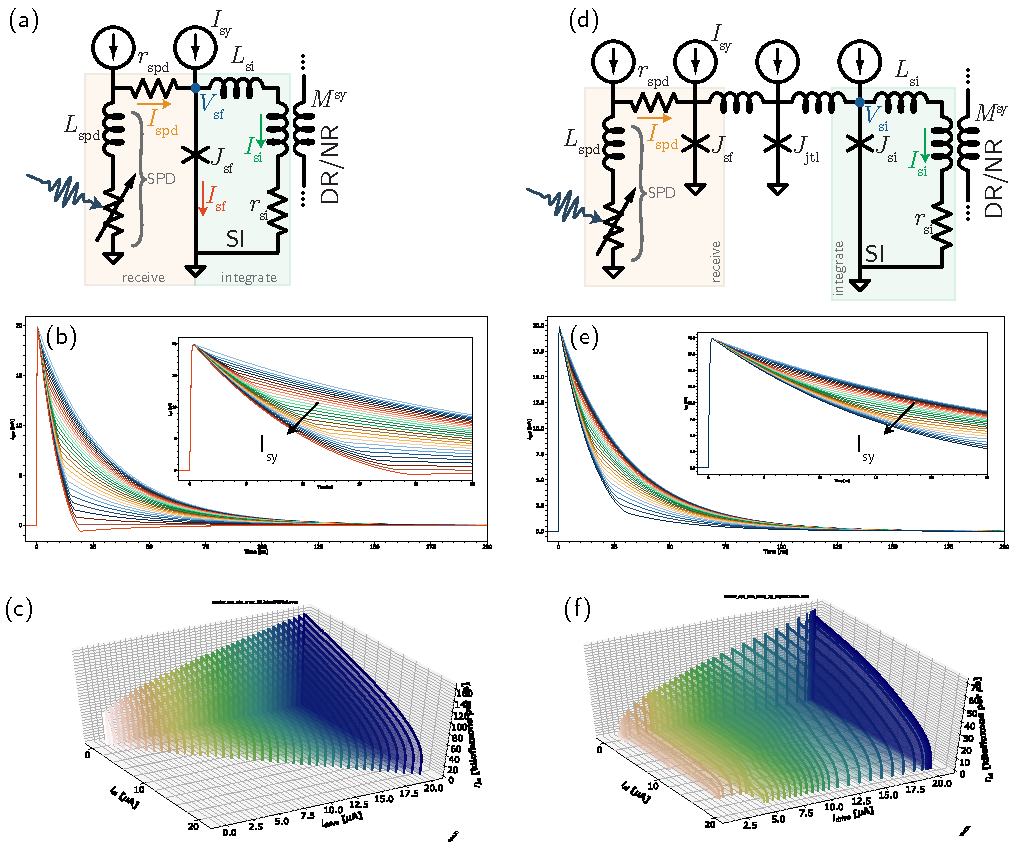
\includegraphics[width=17.2cm]{figures/_fig__synapses__circuits__responses.pdf}
\captionof{figure}{\label{fig:synapses__responses}Caption of fig:synapses circuitsresponses.}
\end{figure*}

\begin{figure*}[h!]
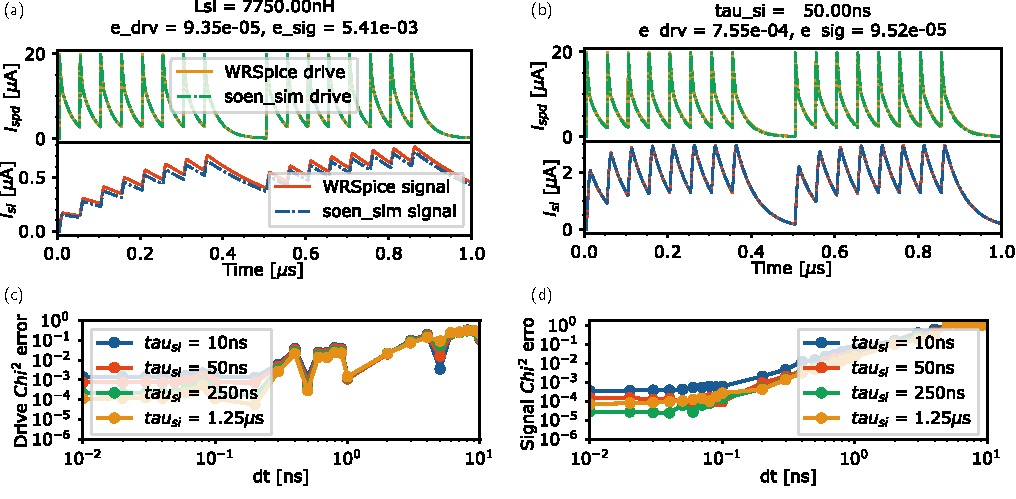
\includegraphics[width=17.2cm]{figures/_fig__synapses__comparison__1jj__main.pdf}
\captionof{figure}{\label{fig:synapses__comparison__1jj__main}Caption of fig:synapses comparison 1jj main.}
\end{figure*}

\begin{figure*}[h!]
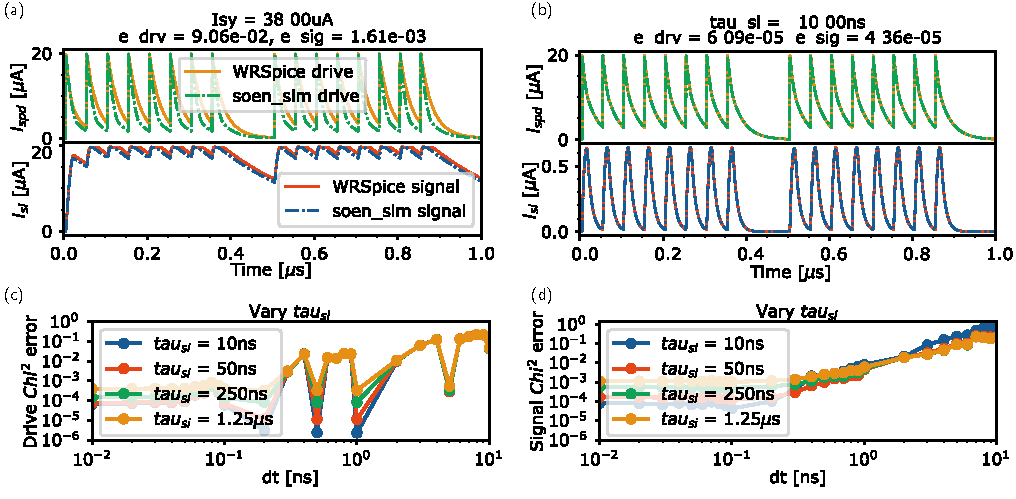
\includegraphics[width=17.2cm]{figures/_fig__synapses__comparison__3jj__main.pdf}
\captionof{figure}{\label{fig:synapses__comparison__3jj__main}Caption of fig:synapses comparison 3jj main.}
\end{figure*}

\cite{amfu1994,fudr2005,fuab2007}

\section{\label{sec:dendrites}Loop Neuron Dendrites as Leaky Integrators}

\begin{equation}
\label{eq:dendrites__leaky_integrator}
\frac{dI^{\mathrm{di}}(t)}{dt} = R_{\mathrm{fq}} \left( \Phi^{\mathrm{dr}}_a(t),I^{\mathrm{di}}(t) \right)\,I_{\mathrm{fq}} - \frac{I^{\mathrm{di}}(t)}{\tau^{\mathrm{di}}}.
\end{equation}
$R_{\mathrm{fq}} \left( \Phi^{\mathrm{dr}}_a(t),I^{\mathrm{di}}(t) \right)$ is the rate function, and $\Phi^{\mathrm{dr}}_a(t)$ is the total applied flux to the dendritic receiving loop:
\begin{equation}
\label{eq:dendrites__applied_flux}
\Phi^{\mathrm{dr}}_a(t) = \sum_i M_i I_i^{\mathrm{si/di}}(t).
\end{equation}
The sum runs over all inputs to the dendritic receiving loop, and the superscript notation $I_i^{\mathrm{si/di}}$ indicates that inputs may be from synaptic or dendritic integration loops.

\begin{figure*}[h!]
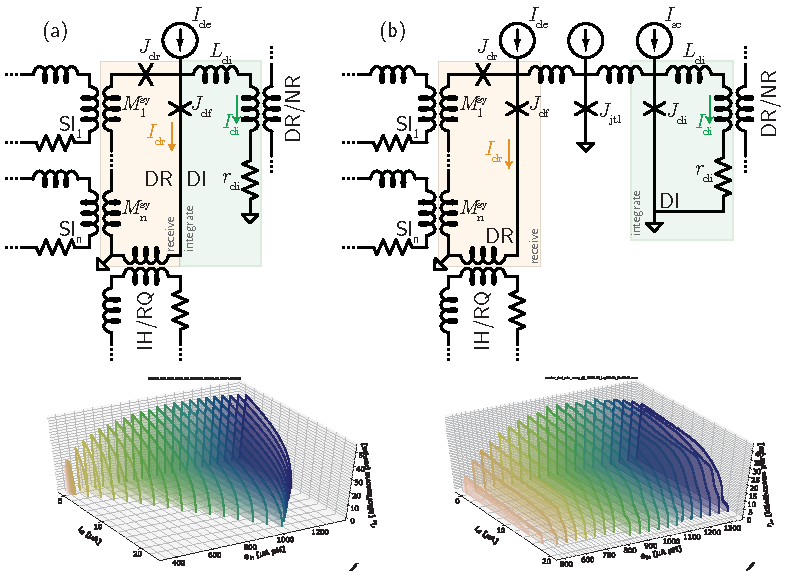
\includegraphics[width=17.2cm]{figures/_fig__dendrites__circuits__responses.pdf}
\captionof{figure}{\label{fig:dendrites__circuits__responses}Caption of fig:dendrites responses.}
\end{figure*}

\begin{figure}[h!]
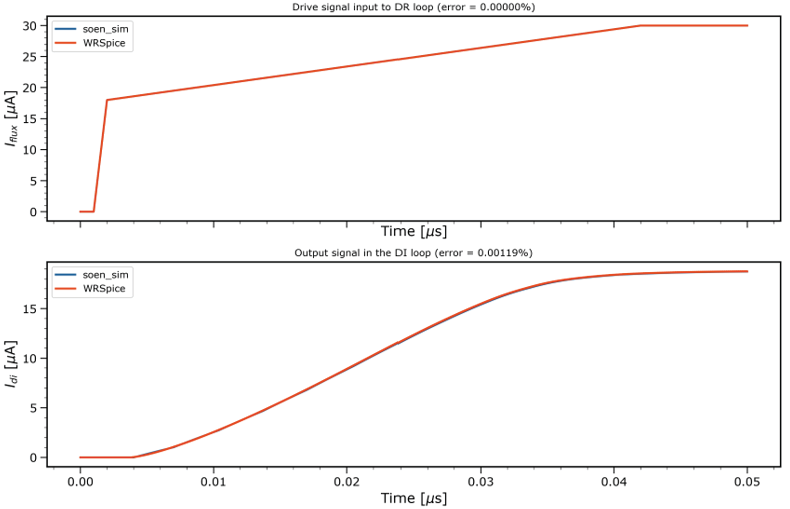
\includegraphics[width=8.6cm]{figures/_fig__dendrites__comparison__2jj__lin_ramp.pdf}
\captionof{figure}{\label{fig:dendrites__comparison__2jj__lin_ramp}Caption of fig:dendrites comparison 2jj lin ramp.}
\end{figure}

\begin{figure}[h!]
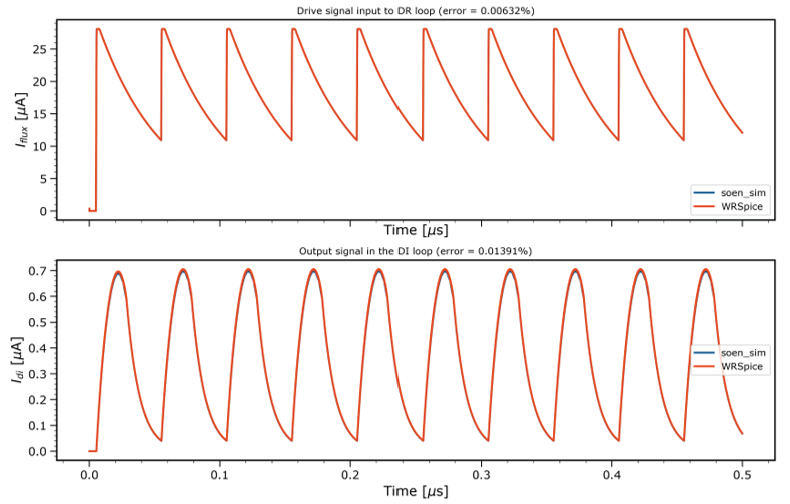
\includegraphics[width=8.6cm]{figures/_fig__dendrites__comparison__2jj__exp_pls_seq.pdf}
\captionof{figure}{\label{fig:dendrites__comparison__2jj__exp_pls_seq}Caption of fig:dendrites comparison exp pls seq.}
\end{figure}

\begin{figure}[h!]
\includegraphics[width=8.6cm]{figures/_fig__dendrites__comparison__2jj__sq_pls_seq.pdf}
\captionof{figure}{\label{fig:dendrites__comparison__2jj__sq_pls_seq}Caption of fig:dendrites comparison sq pls seq.}
\end{figure}

\begin{figure}[h!]
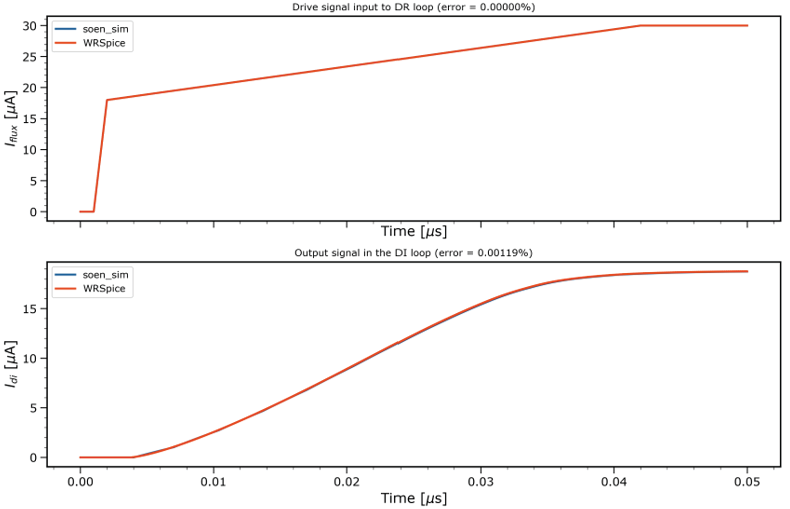
\includegraphics[width=8.6cm]{figures/_fig__dendrites__comparison__4jj__lin_ramp.pdf}
\captionof{figure}{\label{fig:dendrites__comparison__4jj__lin_ramp}Caption of fig:dendrites comparison 4jj lin ramp.}
\end{figure}

\begin{figure}[h!]
\includegraphics[width=8.6cm]{figures/_fig__dendrites__comparison__4jj__sq_pls_seq.pdf}
\captionof{figure}{\label{fig:dendrites__comparison__4jj__sq_pls_seq}Caption of fig:dendrites comparison 4jj sq pls seq.}
\end{figure}

\begin{figure}[h!]
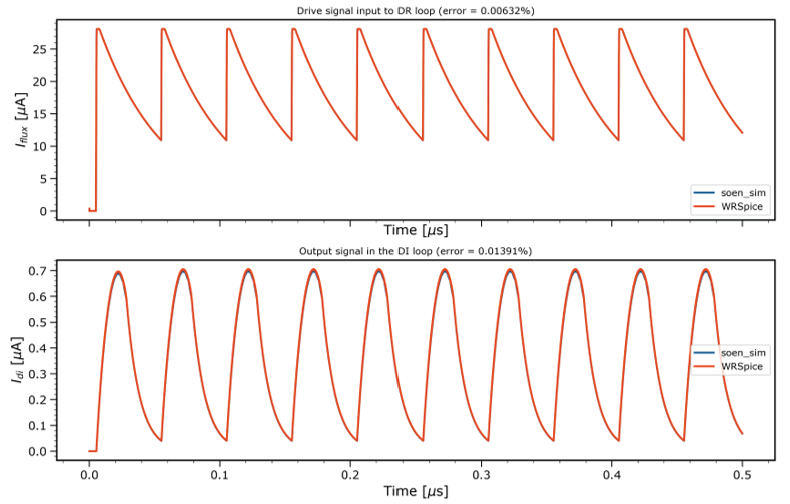
\includegraphics[width=8.6cm]{figures/_fig__dendrites__comparison__4jj__exp_pls_seq.pdf}
\captionof{figure}{\label{fig:dendrites__comparison__4jj__exp_pls_seq}Caption of fig:dendrites comparison 4jj exp pls seq.}
\end{figure}

\begin{figure}[h!]
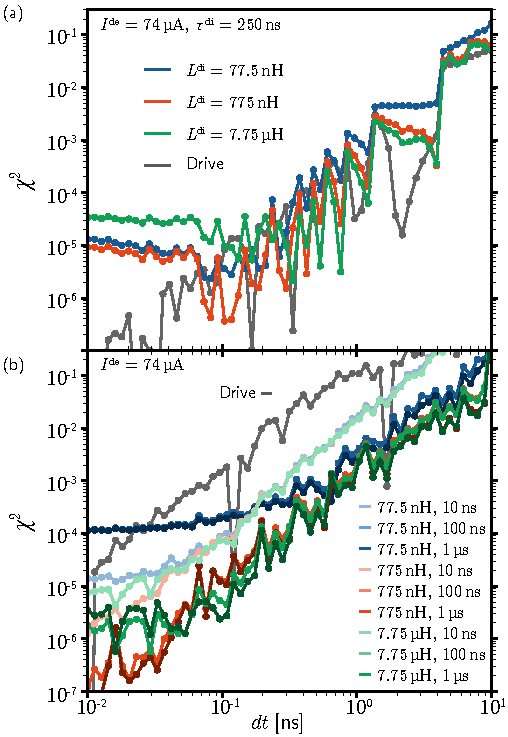
\includegraphics[width=8.6cm]{figures/_fig__dendrites__error_vs_dt__2jj.pdf}
\captionof{figure}{\label{fig:dendrites__error_vs_dt__2jj}Caption of fig:dendrites 2jj error vs dt.}
\end{figure}

\begin{figure}[h!]
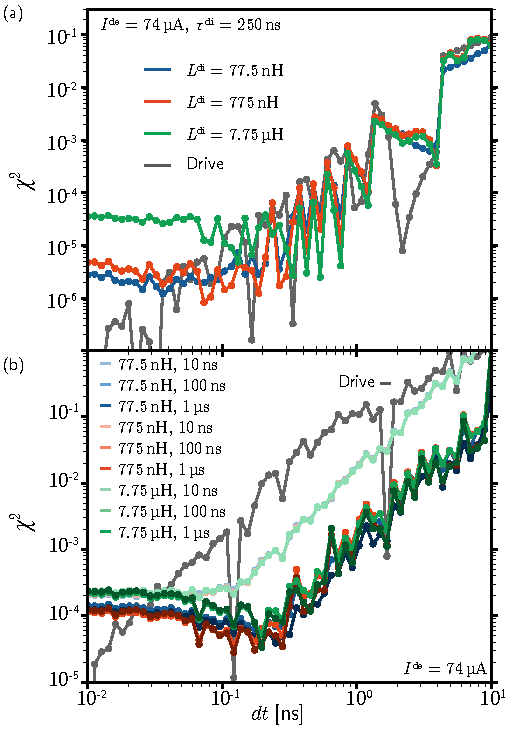
\includegraphics[width=8.6cm]{figures/_fig__dendrites__error_vs_dt__4jj.pdf}
\captionof{figure}{\label{fig:dendrites__error_vs_dt__4jj}Caption of fig:dendrites 4jj error vs dt.}
\end{figure}

\section{\label{sec:neurons}Loop Neurons as Coupled Leaky Integrators}

\begin{figure}[h!]
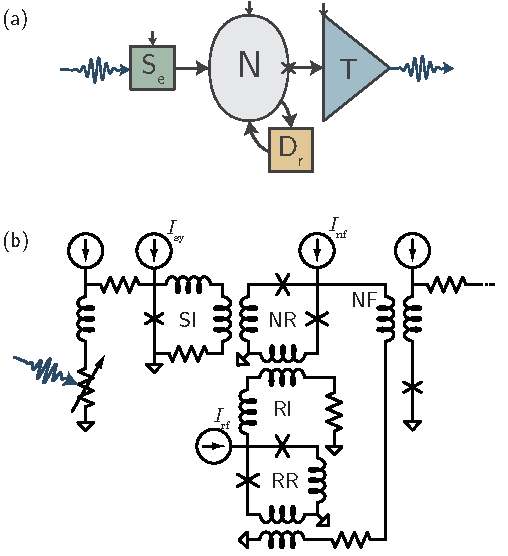
\includegraphics[width=8.6cm]{figures/_fig__point_neuron__one_synapse__schematic__circuit.pdf}
\captionof{figure}{\label{fig:point_neuron__one_synapse__schematic__circuit}Caption of fig:point neuron  one synapse  schematic  circuit.}
\end{figure}

\begin{figure*}[h!]
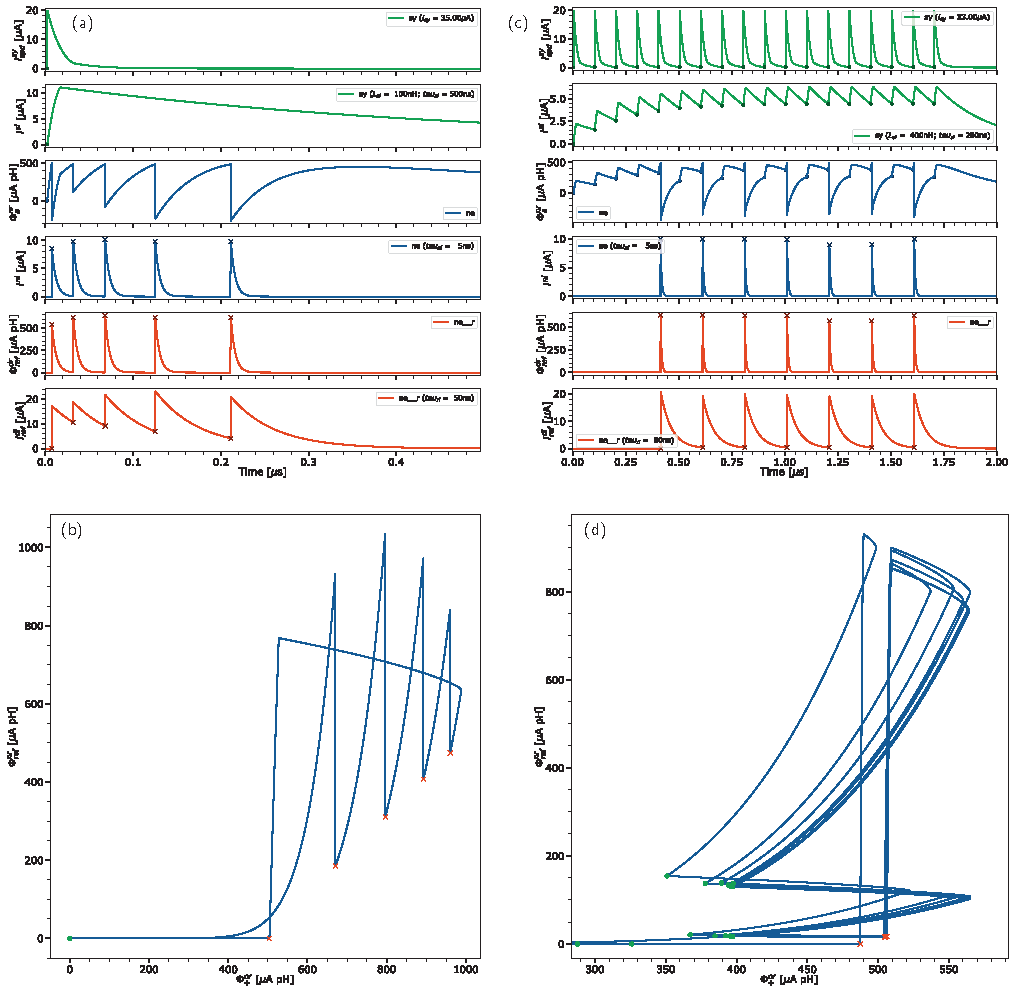
\includegraphics[width=17.2cm]{figures/_fig__point_neuron__one_synapse__data.pdf}
\captionof{figure}{\label{fig:point_neuron__one_synapse__data}Caption of fig:point neuron  one synapse  data.}
\end{figure*}

\begin{figure}[h!]
\includegraphics[width=8.6cm]{figures/_fig__point_neuron__nine_synapses__schematic.pdf}
\captionof{figure}{\label{fig:point_neuron__nine_synapses__schematic__circuit}Caption of fig:point neuron  nine  synapses  schematic.}
\end{figure}

\begin{figure*}[h!]

\includegraphics[width=17.2cm]{figures/_fig__point_neuron__nine_synapses__data.pdf}
\captionof{figure}{\label{fig:point_neuron__nine_synapses__data}Caption of fig:point neuron  nine synapses  data.}
\end{figure*}

\section{\label{sec:discussion}Discussion}

\vspace{1em}
\section{\label{sec:acknowledgements}Acknowledgements}
\noindent This is a contribution of NIST, an agency of the US government, not subject to copyright.

\appendix

\section{\label{apx:synapses}Further data regarding synapse modeling}

\begin{figure*}[h!]
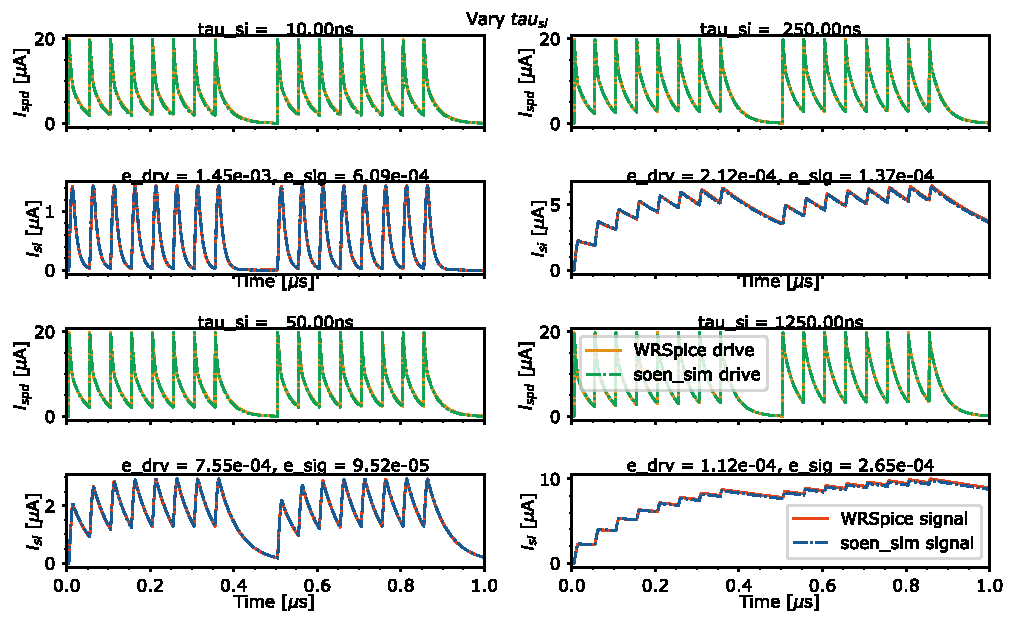
\includegraphics[width=17.2cm]{figures/_fig_apx__synapses__comparison__1jj__tau_si.pdf}
\captionof{figure}{\label{fig:synapses__comparison__1jj__tau_si}Caption of fig:synapses comparison 1jj tau si.}
\end{figure*}

\begin{figure*}[h!]
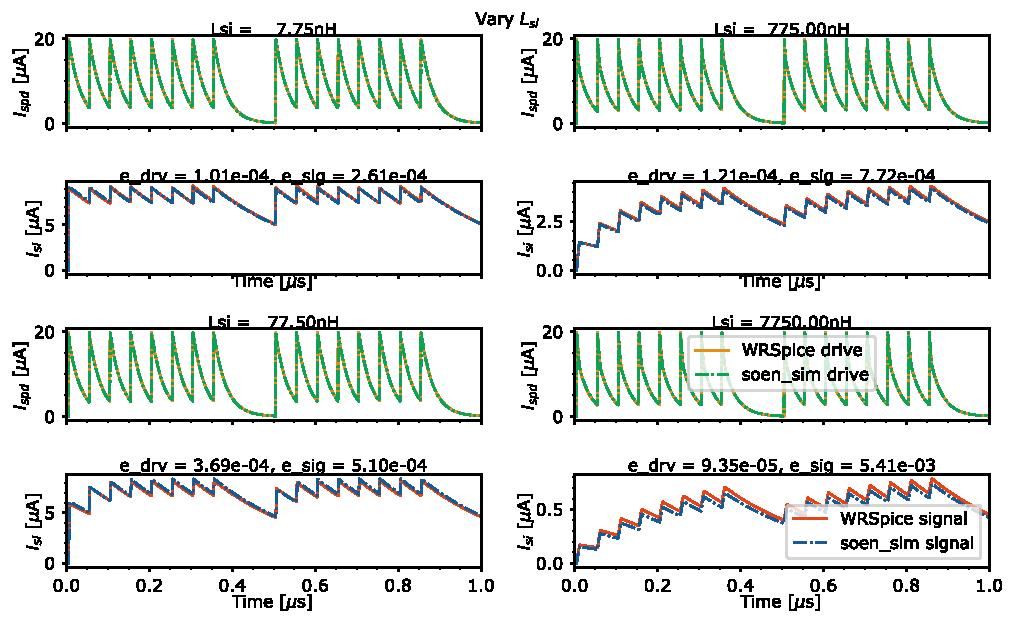
\includegraphics[width=17.2cm]{figures/_fig_apx__synapses__comparison__1jj__L_si.pdf}
\captionof{figure}{\label{fig:synapses__comparison__1jj__L_si}Caption of fig:synapses comparison 1jj L si.}
\end{figure*}

\begin{figure*}[h!]
\includegraphics[width=17.2cm]{figures/_fig_apx__synapses__comparison__1jj__I_sy.pdf}
\captionof{figure}{\label{fig:synapses__comparison__1jj__I_sy}Caption of fig:synapses comparison 1jj I sy.}
\end{figure*}

\begin{figure*}[h!]
\includegraphics[width=17.2cm]{figures/_fig_apx__synapses__error_vs_dt__1jj.pdf}
\captionof{figure}{\label{fig:synapses__error_vs_dt__1jj}Caption of fig:synapses error vs dt 1jj.}
\end{figure*}

\begin{figure*}[h!]
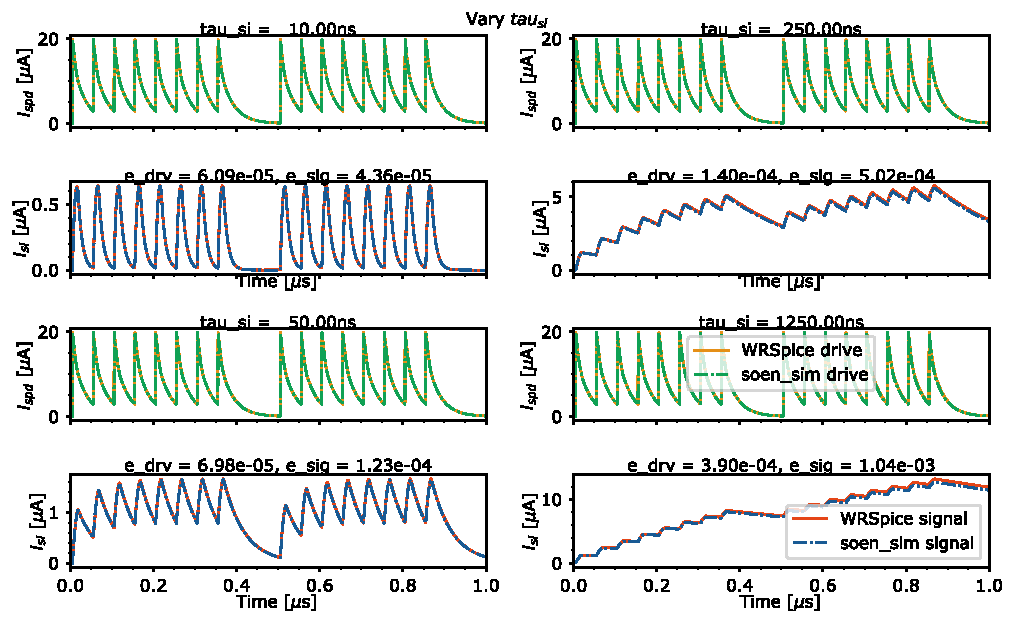
\includegraphics[width=17.2cm]{figures/_fig_apx__synapses__comparison__3jj__tau_si.pdf}
\captionof{figure}{\label{fig:synapses__comparison__3jj__tau_si}Caption of fig:synapses comparison 3jj tau si.}
\end{figure*}

\begin{figure*}[h!]
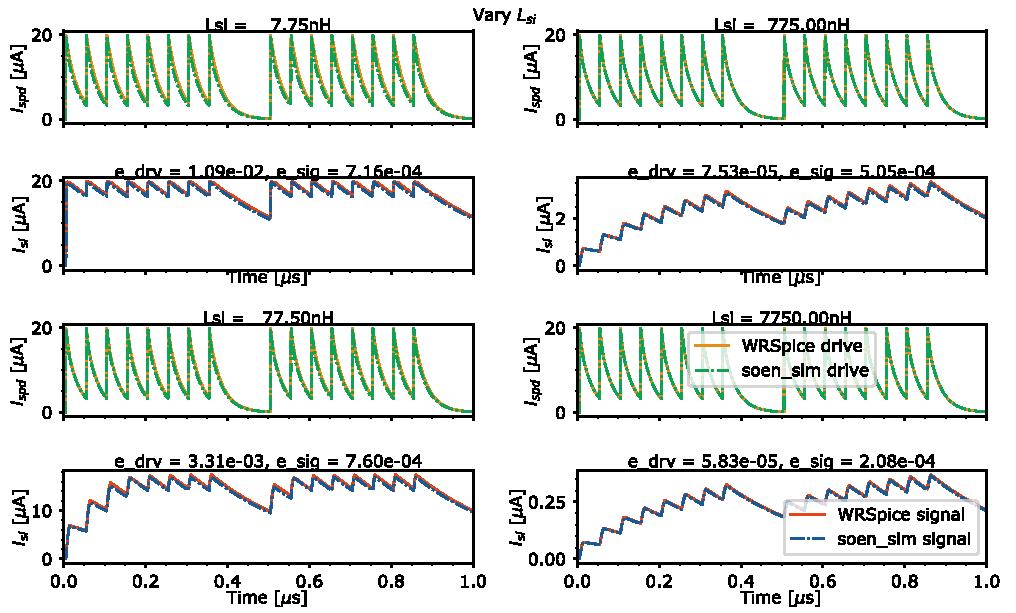
\includegraphics[width=17.2cm]{figures/_fig_apx__synapses__comparison__3jj__L_si.pdf}
\captionof{figure}{\label{fig:synapses__comparison__3jj__L_si}Caption of fig:synapses comparison 3jj L si.}
\end{figure*}

\begin{figure*}[h!]
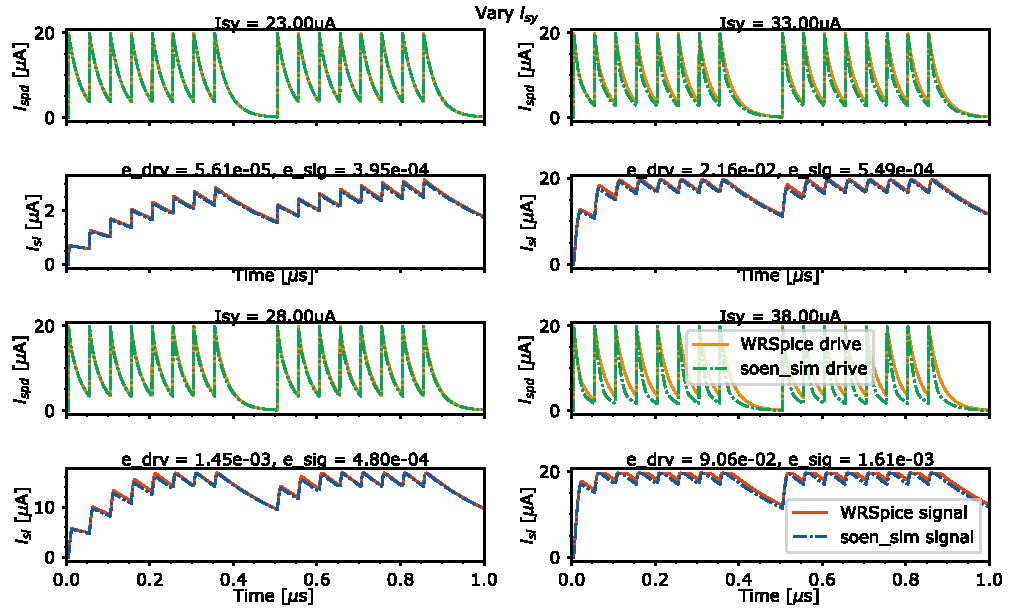
\includegraphics[width=17.2cm]{figures/_fig_apx__synapses__comparison__3jj__I_sy.pdf}
\captionof{figure}{\label{fig:synapses__comparison__3jj__I_sy}Caption of fig:synapses comparison 3jj I sy.}
\end{figure*}

\begin{figure*}[h!]
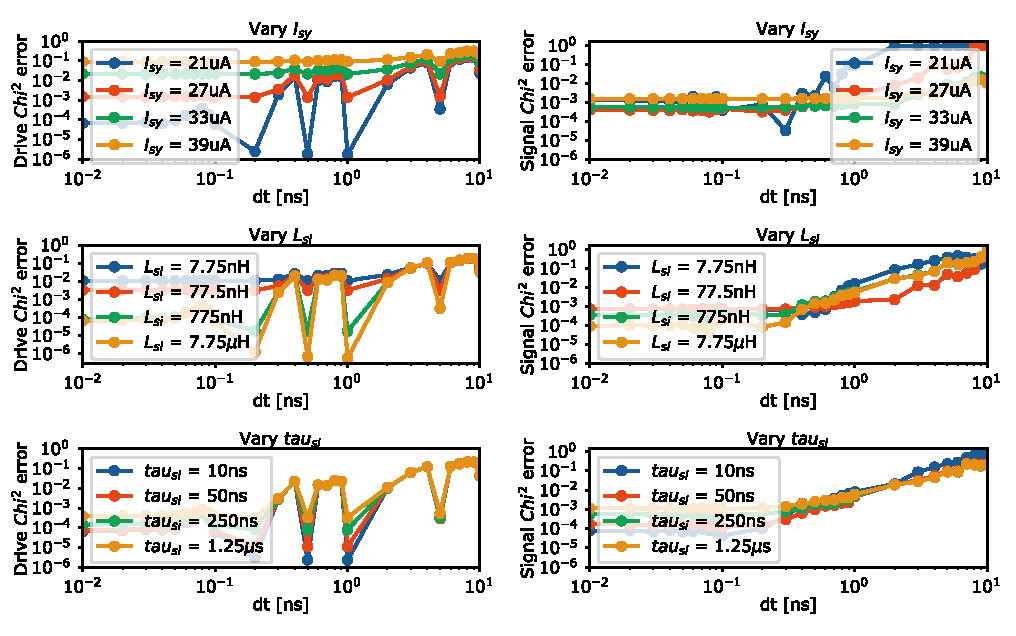
\includegraphics[width=17.2cm]{figures/_fig_apx__synapses__error_vs_dt__3jj.pdf}
\captionof{figure}{\label{fig:synapses__error_vs_dt__3jj}Caption of fig:synapses error vs dt 3jj.}
\end{figure*}

\section{\label{apx:dendrites}Further data regarding dendrite modeling}

\begin{figure}[h!]
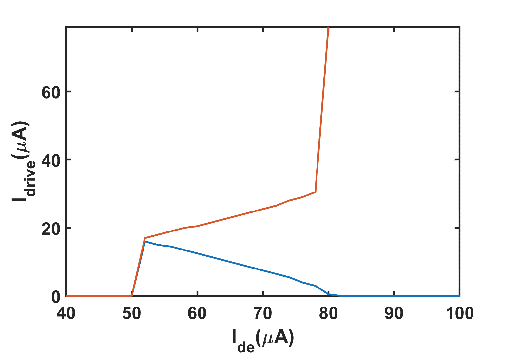
\includegraphics[width=8.6cm]{figures/_fig__dendrites__min_max__2jj.pdf}
\captionof{figure}{\label{fig:dendrites_min_max__2jj}Caption of fig:dendrites min max 2jj.}
\end{figure}

\begin{figure}[h!]
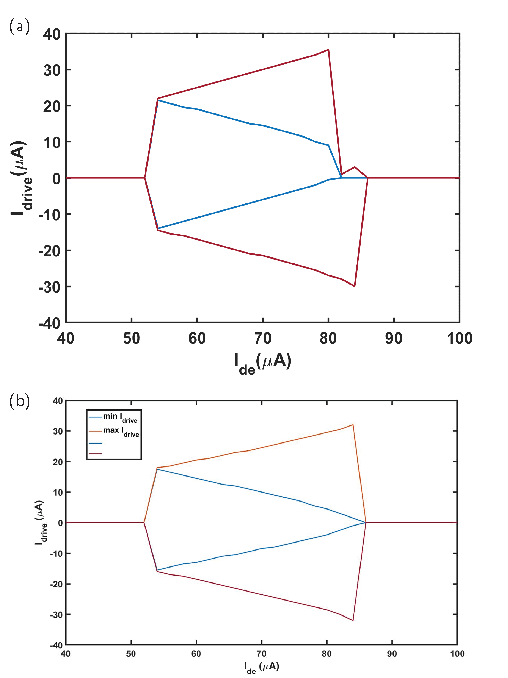
\includegraphics[width=8.6cm]{figures/_fig__dendrites__min_max__4jj.pdf}
\captionof{figure}{\label{fig:dendrites_min_max__4jj}Caption of fig:dendrites min max 4jj.}
\end{figure}

\section{\label{apx:fan_in}Analysis of dendritic and neuronal fan-in}

\begin{figure}[h!]
\includegraphics[width=8.6cm]{figures/_fig__fan-in__circuits.pdf}
\captionof{figure}{\label{fig:fan-in__circuits}Caption of fig:fan-in circuits.}
\end{figure}

We would like to know how to choose the inductors shown in Fig.\,\ref{fig:fan-in__circuits}(a) so the applied flux stays in the appropriate operating range as the number of synaptic connections, $N$, is modified. This consideration will identify the limit of how many synapses can be coupled to a single dendrite or neuron\textemdash the fan-in limit. 

We have seen that the operation of a dendrite (or neuron cell body) is significantly shaped by the inductance of the DR loop. We would therefore like to be able to increase the number of synaptic connections without changing the total inductance of this loop. This total inductance is given by
\begin{equation}
\label{eq:fan-in__direct_input__si_inductance}
L^{\mathrm{nr1}}_{\mathrm{tot}} = \sum_i L^{\mathrm{nr1}}_i = N L^{\mathrm{nr1}}_0
\end{equation}
We would like $L^{\mathrm{nr1}}_{\mathrm{tot}}$ to be independent of $N$, which is possible with $L^{\mathrm{nr1}}_N = L^{\mathrm{nr1}}_0/N$. The total applied flux to the NR loop is given by
\begin{equation}
\label{eq:fan-in__direct_input__applied_flux}
\Phi_{\mathrm{a}}^{\mathrm{nr}} = \sum_i M_i^{\mathrm{si|nr}} \, I_i^{\mathrm{si}}.
\end{equation}
Suppose all SI loops contain a given current, $I_0^{\mathrm{si}}$. We would like the applied flux to the NR loop, $\Phi_{\mathrm{a}}^{\mathrm{nr}}$, to be independent of $N$:
\begin{equation}
\label{eq:fan-in__direct_input__flux_independent_of_N}
\frac{ \Phi_{\mathrm{a}}^{\mathrm{nr}} }{ I_0^{\mathrm{si}} } = \mathrm{cnst.} \neq f(N).
\end{equation}
In the case where all mutual inductors between synapses and the NR loop are equal,
\begin{equation}
\label{eq:fan-in__direct_input__flux_independent_of_N_2}
\frac{ \Phi_{\mathrm{a}}^{\mathrm{nr}}(N) }{ I_0^{\mathrm{si}} } = N\,k\,\sqrt{ L_N^{\mathrm{si2}} \, L_N^{\mathrm{nr1}}},
\end{equation}
where $L_N^{\mathrm{si2}}$ and $L_N^{\mathrm{nr1}}$ are the value ofs $L^{\mathrm{si2}}$ and $L^{\mathrm{nr1}}$ that we should choose for the SI loop output inductor when there are $N$ synapses coupled directly to the NR loop. We have seen above that we need $L_N^{\mathrm{nr1}} = L_0^{\mathrm{nr1}}/N$ to maintain the inductance of the NR loop. Therefore, in order for Eq.\,\ref{eq:fan-in__direct_input__flux_independent_of_N_2} to satisfy Eq.\,\ref{eq:fan-in__direct_input__flux_independent_of_N}, we must also have $L_N^{\mathrm{si2}} = L_0^{\mathrm{si2}}/N$.

This consideration does not explicitly identify a fan-in limit. This limit arises due to practical considerations related to making $L^{\mathrm{si2}}$ and $L^{\mathrm{nr1}}$ exceedingly small as $N$ grows large. With $L_0 \approx 1$\,pH a rough lower limit on what we would like to fabricate, and $L_{\mathrm{tot}}^{\mathrm{nr}} \approx 20$\,pH, we see direct fan-in with this circuit design is limited to about 20. This limit can be straightforwardly overcome with an intermediate transformer collection coil, as shown in Fig.\,\ref{fig:fan-in__circuits}(b).

\begin{equation}
\label{eq:fan-in__transformer_collection}
\frac{\Phi_{\mathrm{a}}^{\mathrm{nr}}}{I_0^\mathrm{si}} \approx \frac{ M^{\mathrm{si|nt}} \, M^{\mathrm{nt|nr}} }{L^{\mathrm{nt1}}} \left( 1-\epsilon \right) + \mathcal{O}(\epsilon^2)
\end{equation}
$M^{\mathrm{si|nt}} = k\sqrt{L^{\mathrm{si2}} \, L^{\mathrm{nt1}}}$ and $M^{\mathrm{nt|nr}} = k\sqrt{L^{\mathrm{nt3}} \, L^{\mathrm{nr1}}}$

\begin{equation}
\label{eq:fan-in__transformer_collection__epsilon}
\epsilon \equiv \frac{ L^{\mathrm{nt2}}+L^{\mathrm{nt3}} }{ N L^{\mathrm{nt1}} }
\end{equation}


\bibliographystyle{unsrt}
\bibliography{phenomenological_modeling}

\end{document}